\documentclass{article}
\usepackage[utf8]{inputenc}
\usepackage[ngerman]{babel}
\usepackage{csquotes}
\usepackage[ngerman=ngerman-x-latest]{hyphsubst}
\usepackage{color} %Zum stylen von \def
\usepackage{varwidth} %Zum stylen von \def
\usepackage{etoolbox} %Zum stylen von \def
\usepackage{amssymb} %Für die Mengensymbole
%\usepackage{svg}
\usepackage{graphicx}
\graphicspath{ {./images/} }
\usepackage{amsmath} %Zur Darstellung von Funktionen mit Fallunterscheidung
\usepackage{scrlayer-scrpage} %Kopf- und Fusszeile
\usepackage{titling} %Titel nach oben verschieben
\usepackage{amsfonts} %\mathcal
\usepackage{enumerate} %Für kleine römische Zahlen in Aufzählungen
\usepackage{hyperref}
\usepackage[normalem]{ulem} %für durchgestrichenen text
\newcommand{\stkout}[1]{\ifmmode\text{\sout{\ensuremath{#1}}}\else\sout{#1}\fi} %text durchstreichen auch in math-mode

%\usepackage{prettyref}
%\usepackage{apacite}
\usepackage[
backend=biber,
style=apa,
]{biblatex}
\addbibresource{references.bib}

%\usepackage{array,multirow}



%% Formatierung %%
\sloppy
\usepackage[dvipdfm]{geometry}
\setlength{\droptitle}{-10em}
\geometry{bottom=3.5cm, textwidth=15cm, headsep=15mm, top=5cm,head=15pt}
%%%%%%%%%%%%%%%%%%

%\usepackage{vaucanson-g}
%%  Kopf- und Fusszeile anpassen %%
\pagestyle{scrheadings} 

\ihead{\small{Bachelorarbeit}}
\ohead{\small{Sebastian Flick, Universität Bern}}
\cfoot{\thepage}
%%%%%%%%%%%%%%%%%%%%%%%%%%%%%%%%%%%

\newcounter{std}
\setcounter{std}{1}

%% New Commands %%
\newcommand{\comment}[1]{{\color{red} #1}}

\definecolor{bg}{gray}{1}
\newcommand{\spec}[3]{
    \begin{flushleft}
    \mpar{\vspace{.5cm}#2}\colorbox{bg}{\hspace{.4cm}\parbox{\textwidth}{
        \begin{varwidth}{\dimexpr\linewidth-2\fboxsep}
            \vspace*{.2cm}
            \noindent{\textbf{#1 \ifstrempty{#2}{}{\textit{#2}: }}#3}
            \stepcounter{std}
        \end{varwidth}
    }}
    \end{flushleft}
}

\newcommand{\formula}[1]{\\$#1$}

\renewcommand{\L}{\Box}
\newcommand{\M}{\Diamond}
\newcommand{\qed}{\hspace{0.5cm}$\blacksquare$}

\newcommand\mpar[1]{\marginpar {\flushleft\sffamily\small #1}}
\setlength{\marginparwidth}{2cm}

%%%%%%%%%%%%%%%%%%%%

\newcommand{\R}{\mathbb{R}}
\newcommand{\Z}{\mathbb{Z}}
\newcommand{\N}{\mathbb{N}}
\newcommand{\C}{\mathbb{C}}

\newcommand{\bmt}{\begin{pmatrix}}
\newcommand{\emt}{\end{pmatrix}}

\title{Ein realistischeres Modell des Reflective Equilibrium}
\author{Bachelorarbeit von Sebastian Flick, 16-121-014\\Betreut von Prof. Dr. Dr. Claus Beisbart\\Universität Bern}


\date{\today}

\begin{document}
\maketitle
\section{Einführung}
In dieser Arbeit geht es um ein Modell, welches das Überlegungsgleichgewicht umsetzt. Für diese Methode zur Rechtfertigung, welches seit den Siebzigerjahren des letzten Jahrhunderts von vielen Philosophen vertreten und von ähnlichen vielen kritisiert wurde, entwickelten \citeauthor{beisbart_making_2015} nämlich ein exaktes Modell.
Das Ziel der Arbeit ist es, innerhalb dieses Modells einen kleinen, aber wichtigen Aspekt zu untersuchen: die Theorie- und Überzeugungsanpassung. Konkret soll ein Piecemeal-Ansatz formuliert werden. Dieser soll Anpassung von Überzeugungen und Theorien umsetzbarer und nachvollziehbarer zu machen. Um herauszufinden, wie Theorien und Überzeugungen in den jeweiligen Anpassungsschritten angepasst werden müssen, wird bisher einfach jede mögliche und konsistente Kombination von Prinzipien bzw. Überzeugungen überprüft. Dies ist einerseits nicht, was \citeauthor{goodman_fact_1983} im Sinn hatte, als er Reflective Equilibrium beschrieb - er sprach von einzelnen Sätzen, welche zur Theorie bzw. zu den Überzeugungen addiert oder subtrahiert würden \autocite{goodman_fact_1983}, andererseits ab einer gewissen Grösse des zu behandelnden Themas schlicht nicht umsetzbar. Ausserdem ist es wichtig einen intuitiven Weg zu finden, wie die Änderungen an Theorie und Überzeugungen gemacht werden - Denn auch von diesem Faktor hängt die Glaubwürdigkeit der Methode ab. Ein möglicher Weg ist ein Piecemeal-Ansatz, welcher Überzeugungen und Prinzipien stückweise zu vorhanden Überzeugungen bzw. Theorien hinzufügt. Ich setze mir zum Ziel, einen bestimmten Piecemeal-Ansatz auszuformulieren. Wenn in der Folge der Arbeit von einem Piecemeal-Ansatz die Rede ist, ist mein ausformulierter Ansatz gemeint. Um herauszufinden, ob sich die Anwendung des Piecemeal-Ansatzes lohnt, werde ich eine Ensemblestudie generieren und die vorhandenen Daten analysieren, um zu verstehen, unter welchen Bedingungen der Piecemeal-Ansatz tatsächlich besser ist, als der traditionelle Ansatz.

Ich werde zum Beginn der Arbeit die Methode Reflective Equilibrium vorstellen und eine kleine historische Einführung in das Thema geben. Danach werde ich den Piecemeal-Ansatz detailliert vorstellen. Ich werde sie innerhalb des Modells von \citeauthor{beisbart_making_2015} definieren und zeigen, dass der Ansatz unter bestimmten Bedingungen besser ist als der konventionelle. Ausserdem werde ich einen Vorschlag für die Erstellung einer ersten Theorie vorbringen.

\section{Reflective Equilibrium und seine Ursprünge}

Bei Reflective Equilibrium handelt es sich um eine Methode zur Rechtfertigung unserer Überzeugungen. Sie ist durchaus als alltägliches Instrument zu verstehen, das jede Person nutzt, um zu gerechtfertigter Meinung zu kommen. Wir pflegen unsere Festlegungen in ein System von Prinzipien ein und passen beides aneinander an. Am Ende dieser Anpassungen erhalten wir einen Gleichgewichtszustand. Aus dem System von Prinzipien folgen - einige oder alle - unsere Überzeugungen, die wir anfangs für plausibel hielten. Dadurch ist die Überzeugung gerechtfertigt. Es gibt verschiedene Auffassungen darüber, wie Reflective Equilibrium funktioniert - oder funktionieren soll - und wie es zu verstehen ist \autocite{sep-reflective-equilibrium}.
Ich werde mich in dieser Arbeit aber vor allem an die Interpretation, die auch in \cite{beisbart_making_2015} vertreten wird, halten. Dies beinhaltet, dass Reflective Equilibrium - wie eingangs beschrieben - durchaus eingesetzt werden kann zur Beantwortung von Fragen in einem Gebiet und somit nach Scanlon deliberativ ist. Eine rein deskriptive Auffassung, bei welcher durch das Reflective Equilibrium lediglich herausgefunden werden kann, welche Überzeugungen eine Person hat \autocite[S.~143]{freeman_rawls_2002}. Für Scanlon ist der Prozess kein rein quantitatives Unterfangen. Das Individuum, welches einen RE-Prozess durchführt, merkt beispielsweise durch welche Prinzipien ihr Commitment gestützt wird und kann sich dann spontan dazu entscheiden, das Commitmentment aufzugeben. Für ihn ist somit ausgeschlossen, dass der Prozess durch ein mathematisches Modell abgebildet werden kann. \autocite[S.~148]{freeman_rawls_2002}
Eine weitere Distinktion in den verschiedenen Interpretationen von Reflective Equilibrium, ist die Unterscheidung zwischen \textit{wide} (breit) und \textit{narrow} (schmal) Reflective Equilibrium: Diese wurde von \citeauthor{daniels_wide_1996} ins Spiel gebracht. Das Modell von \citeauthor{beisbart_making_2015} bildet ein \textit{narrow} RE ab. Denn für bei einem \textit{wide} RE würden Hintergrund-Theorien miteinbezogen werden und diesen wurde im Modell kein Platz eingeräumt. Hintergrundtheorien können während des Prozesses nicht verändert werden und geniessen einen Sonderstatus. Durch eine Einschränkung der Argumente - diese müssen mit etwaigen Hintergrundtheorien konsistent sein - könnte das Modell aber auch innerhalb eines \textit{wide} RE funktionieren. \autocite[S.~22]{beisbart_making_2015}

Der Begriff Reflective Equilibrium wurde 1971 von John Rawls geprägt. In \autocite{rawls_theory_1971} erarbeitet er die Methode, um die \textit{original position} einer Gesellschaft zu rechtfertigen. In dieser überprüft man, ob die gewählten Prinzipien mit den in Betracht gezogenen Überzeugungen (betreffend der Gerechtigkeit) übereinstimmen oder diese in akzeptierbarer Weise erweitern. Wir haben gewisse Überzeugungen (über Gerechtigkeit) für die wir klare Intuitionen haben. Diese Überzeugungen können wir als Fixpunkte benutzen, um mit Prinzipien, welche diese Fixpunkte erklären, weitere Überzeugungen zu erklären, für die wir keine klaren Intuitionen haben. Durch die Beschreibung der \textit{initial situation} generieren wir Prinzipien, diese gleichen wir mit den Überzeugungen ab. Erklären die Prinzipien die Überzeugungen nicht, so kann man entweder die Überzeugungen anpassen oder aber die Prinzipien. Daraus entsteht - nach möglicherweise mehrmaliger Wiederholung - ein Reflective Equilibrium. Er beschreibt die Überzeugungen und Theorie als jeweils eine Einheit, diese werden auch als Einheit verändert. Ein Piecemeal-Ansatz - wie ich ihn später als Alternative vorschlagen werde - ist bei Rawls also nicht zu entdecken. Rawls verweist bei der Verwendung des Begriffs Reflective Equilibrium auf \cite{goodman_fact_1983}, welcher vor ihm über die Idee gesprochen hat, ihr aber noch keinen Namen gegeben hat. \autocite[S.~20]{rawls_theory_1971}

Bei Goodman ist ein Piecemeal-Ansatz, bei dem Theorie und Überzeugungen stückweise angepasst werden, zu entdecken:

\begin{quote}
    A rule is amended if it yields an inference we are unwilling to accept; an inference is rejected if it violates a rule we are unwilling to amend. \autocite[S.~64]{goodman_fact_1983}
\end{quote}

Er spricht also von einzelnen Prinzipien, welche abgeändert werden, statt von einer ganzen Theorie. Und von einzelnen Überzeugungen, die angepasst werden, wenn sie einem Prinzip widersprechen, dass wir nicht ändern wollen. Nicht alle Autoren, die sich zum Thema Reflective Equilibrium äussern, machen sich detaillierte Gedanken über die Anpassungsschritte. So scheint es beispielsweise bei \autocite{tersman_reflective_1993} unklar, ob er sich für einen Piecemeal-Ansatz ausspricht oder nicht. Wohl einfach, weil es nicht im Fokus seiner Arbeit lag. Es soll aber im Fokus der vorliegenden Arbeit liegen. Dazu fasse ich zuerst kurz das Model in \citeauthor{beisbart_making_2015} kurz vor und lege den Fokus auf die Änderungen an einem System, da dies der Teil ist, der uns am meisten interessiert.

\section{Das konventionelle System}

Das Modell von \citeauthor{beisbart_making_2015} geht von einer Menge von Sätzen aus, die für das Thema, über welches man ein RE erhalten will, relevant sind. Diese Menge ist unter Negation geschlossen. Das heisst, wenn sie einen Satz beinhalten, so beinhaltet sie auch dessen Negation.
Der Prozess, welcher abgebildet wird, beginnt mit einem initialen epistemischen Zustand.

\paragraph{Der epistemische Zustand} Dieser epistemische Zustand besteht aus Theorie und einer Menge von Überzeugungen. Die Theorie wiederum besteht aus einzelnen Prinzipien. Prinzipien können beliebige Sätze aus der Satzmenge sein. Der Inhalt einer Theorie ist die Menge von Sätzen, die aus den Prinzipien folgt. So kann nun also jeder Satz in einem Satzpool Prinzip, Inhalt und/oder Überzeugung sein. Sätze folgen aus sich selbst, sodass im Inhalt einer Theorie immer auch die Prinzipien sind. In Abbildung \ref{fig:smallset} ist die Menge aller Sätze folgende: $\{s1,s2,\neg s1, \neg s2\}$. Durch den Pfeil ist angedeutet, dass $s2$ aus $s1$ folgt. Dies ist das einzige Argument in der Struktur. Zum initialen Zustand gehört nun also eine Menge von Überzeugungen. Wir wählen $\{s2\}$. Ausserdem gehört eine initiale Theorie dazu. Diese ist im Standard-Modell die leere Menge. Der Inhalt der leeren Menge ist ebenfalls die leere Menge - Das heisst aus der leeren Menge folgen keine Sätze. Angenommen $\{s1\}$ wäre die Theorie, so wäre $s1$ das einzige Prinzip der Theorie und $\{s2\}$ der Inhalt der Theorie.

Hat man einen initialen epistemischen Zustand, folgt als erster Schritt die Änderung der Theorie und danach die Änderung der Überzeugungen. Diese werden so lange angewendet, bis eine Haltebedingung zutrifft.\autocite[S.~10]{beisbart_making_2015}

Für die Änderung der Theorie werden verschiedene Theoriekandidaten miteinander verglichen. Ich werde \textit{\textcolor{red}{später}} darauf zu sprechen kommen, wie diese gefunden werden. Die Kandidaten werden mittels einer Achievement-Funktion überprüft.

\paragraph{Die Achievement-Funktion} \label{achievement-funktion}
Die Achievement-Funktion untersucht einen epistemischen Zustand auf die Kriterien der \textit{Kohärenz (Account)}, der \textit{Systematizität (Systematicity)} und des \textit{Respekts (Faithfulness)}. \textit{Kohärenz} beschreibt, wie sehr die Theorie die Überzeugungen erklärt. Dabei wird der Wert der Kohärenz verringert, für jede Überzeugung, welche mit der Theorie inkonsistent ist, für jede, die nicht im Inhalt der Theorie ist und für jeden Satz im Inhalt der Theorie, welcher keine Überzeugung ist. Vor allem dieser letzte Punkt scheint etwas kontraintuitiv. Warum sollte es schlechter für die Kohärenz sein, wenn eine Theorie mehr erklärt, als die gesuchten Überzeugungen? \citeauthor{beisbart_making_2021} erklären dies damit, dass dies einen Druck dahingehend erzeugt, dass die Überzeugungen alle Sätze im Inhalt der Theorie bei den Anpassungsschritten der Überzeugungen aufnehmen.
\textit{Systematizität} bezieht sich nur auf die Theorie eines epistemischen Zustandes. Je mehr Sätze im Inhalt einer Theorie sind im Verhältnis zu den Sätzen in der Theorie, umso systematischer ist die Theorie. Eine Theorie mit einem Satz, welcher vier Sätze im Inhalt der Theorie hat, ist also systematischer, als eine Theorie, mit einem Satz, welche nur sich selbst im Inhalt der Theorie hat.
\textit{Respekt} bezieht sich nur auf die Überzeugungen eines epistemischen Zustandes. Der Respekt der Überzeugungen wird schlechter, für jede initiale Überzeugung, welche negiert in den Überzeugungen vorkommt und für jede initiale Überzeugung, die nicht vorkommt.

\paragraph{Gewichtung} Diese drei Desiderata sind unterschiedlich gewichtet. Dies ist wichtig, da die Desiderata einen epistemischen Zustand oft in unterschiedliche Richtungen ziehen. Beispielsweise wird ein epistemischer Zustand kohärenter, wenn man alle Überzungen entfernt, die nicht Teil des Inhalts sind. Darunter leidet allerdings der Respekt. Deshalb müssen die Desiderata unterschiedlich gewichtet werden, damit überhaupt Fortschritt erzielt werden kann. Ich verwendete für meine Ensemblestudie lediglich die Standard-Gewichte (Kohärenz: 0.35, Respekt: 0.10, Systematizität: 0.55) und werde innerhalb der Arbeit auch nicht weiter auf die Gewichte eingehen. Es sei lediglich vermerkt, dass das Modell verschiedene Gewichtungen der Desiderata erlaubt. \autocite[S.~9]{beisbart_making_2015}

\paragraph{Konsistenz\label{konsistenz}}
Ich habe bisher den Begriff der Konsistenz schon einige mal verwendet, ohne genau zu definieren, was dieser bedeutet. Das möchte ich nun ändern. Konsistenz bedeutet in der Logik, dass eine Menge von Sätzen gleichzeitig wahr sein kann. Dass also aus ihr kein Widerspruch abgeleitet werden kann. In dieser Arbeiten spielen zwei Arten der Konsistenz eine Rolle: minimale Konsistenz und volle Konsistenz. Bei der minimalen Konsistenz wird lediglich gefordert, dass die Menge von Sätzen nicht einen Satz und gleichzeitig dessen Negation enthält. Bei voller Konsistenz, welche von Theorien gefordert wird, werden die inferenziellen Beziehungen von Sätzen miteinbezogen. Wenn also bspw. der Satz $s3$ aus $s1$ folgt und aus $s2$ folgt $\neg s3$, so wäre die Menge von Sätzen ${s1,s2}$ inkonsistent, denn aus ihr folgt $s3$ und $\neg s3$ und dies ist ein Widerspruch. Siehe dazu Abbildung \ref{fig:inconsistency}. Anders ausgedrückt kann man auch sagen, dass wenn von einer Theorie volle Konsistenz gefordert wird, so wird von Ihrem Inhalt minimale Konsistenz gefordert. Im Inhalt dürfen sich keine Sätze finden, deren Negationen sich auch darin finden.

\begin{figure}[ht]
  \centering
  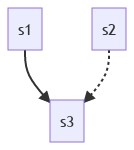
\includegraphics{consistence.png}
  \caption{Möglichkeit der Inkonsistenz\label{fig:inconsistency}}
\end{figure}

Wenn Überzeugungen im Modell von \citeauthor{beisbart_making_2015} angepasst werden müssen, so funktioniert dies nach einem einfach beschriebenen Rezept:

\begin{quote}
    [...] the agent replaces her current commitments $C_i$ with those commitments $C_{i+1}$ that score best on the achievement function Z (given $T_{i+1}$).
    \autocite[S.~11]{beisbart_making_2015}
\end{quote}

Die Menge von Überzeugungen, welche (zusammen mit der aktuellen Theorie) den höchsten Wert der \textit{Achievement-Funktion} $Z$ erreicht, wird als neue Menge von Überzeugungen übernommen. Aber welche Mengen von Überzeugungen ($C^*$) stehen uns überhaupt zur Verfügung? Die Anzahl der Mengen von Überzeugungen in $C^*$ ($\lvert C^* \lvert$) ist aus der Menge an Sätzen im Thema bestimmt. Je mehr Sätze, umso mehr Mengen von Überzeugungen. Das Problem ist, dass $\lvert C^* \lvert$ exponentiell zur Zahl der Sätze im Thema wächst. Jeder zusätzliche Satz in einem Thema verdreifacht die Anzahl der Mengen von Überzeugungen. Das kommt daher, dass ein Satz oder seine Negation Teil einer Menge von Überzeugungen sein kann oder er ist nicht dabei. Das sind pro Satz 3 Möglichkeiten. Aus diesen Überlegungen leitet sich die Zahl der zu überprüfenden Mengen von Überzeugungen pro Anpassungsschritt ab: $\lvert C^* \rvert = 3^n$, wobei $n$ die Zahl der Sätze im Thema ist. Es gilt zu beachten, dass noch mehr als 3 Möglichkeiten pro neuen Satz bestehen: Es könnte ja auch der Satz und seine Negation Teil einer Menge von Überzeugungen sein. Diese Möglichkeit wird aber ausgeschlossen, da von Mengen von Überzeugungen \textit{minimale Konsistenz} gefordert wird.

Die Regel zur Anpassung einer Theorie sieht zwar analog aus, allerdings können die Sätze, welche überprüft werden müssen, etwas eingeschränkt werden.

\begin{quote}
    [...] the agent newly adopts an epistemic state $(C_i, T_{i+1})$ such that the theory $T_{i+1}$ scores best in terms of the achievement function $Z$ given $C_i$.
    \autocite[S.~11]{beisbart_making_2015}
\end{quote}

Zusätzlich schränken nun die Inferenzbeziehungen zwischen den Sätzen, die Kandidaten ein. Weil Theorien vollständig konsistent sein müssen, darf auch kein Theoriekandidat Inkonsistenzen enthalten.
Im traditionellen Ansatz werden inkonsistente Mengen vorneweg ausgeschlossen, um später nicht immer wieder einzeln die Konsistenz prüfen zu müssen. Deshalb wird vorab der Inhalt jeder möglichen Theorie ($3^n$) errechnet und abgespeichert. Alle Mengen mit Inhalten, die Widersprüche enthalten, werden ausgeschlossen. Dies bedeutet aber auch, einen zusätzlichen Mehraufwand, weil über alle möglichen Theorien iteriert werden muss.

Für eine sehr kleine Menge von Sätzen gelingt eine übersichtliche Darstellung der Theoriekandidaten noch. Bei Abbildung \ref{fig:smallset} ist eine sehr kleine Menge von Sätzen abgebildet. Wenn nun \textit{s2} die einzige Überzeugung ist und man dazu die passende Theorie suchen möchte, so würden folgende Kombinationen überprüft: $\{\{\}, s1, s2, \neg s1, \neg s2, \{s1,s2\}, \{s1,\neg s2\}, \{\neg s1, s2 \}, \{\neg s1, \neg s2 \} \}$. In dieser einfachen Struktur können keine Mengen ausgeschlossen werden. Alle 9 Elemente müssten überprüft werden. Wenn nun ein einziges weiteres Element \textit{s3} hinzukäme, müssten 27 Mengen überprüft werden. Bei einem weiteren 81. Das heisst, der Arbeitsaufwand wächst exponentiell zur Anzahl an Sätzen im System. Dies macht diese Methode unrealistisch in der Benutzung. Ausserdem ist es auffällig, wie schnell und einfach die Anpassung intuitiv gemacht werden kann. Für eine Person ist es auf einen Blick zu erkennen, dass s1 das einzige Prinzip ist, welches infrage kommt. Deshalb muss ein neuer Ansatz entwickelt werden.

\begin{figure}[ht]
  \centering
  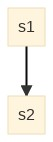
\includegraphics{figure1}
  \caption{Eine kleine Menge von Sätzen\label{fig:smallset}}
\end{figure}

\section{Der piecemeal Ansatz} \label{piecemealansatz}
Wie \autocite[S.25]{beisbart_making_2015} feststellten, scheint die naheliegendste und einfachste Umsetzung eines Piecemeal-Ansatzes zu sein, einzelne Überzeugungen oder Prinzipien in einer vorhandenen Theorie bzw. Menge von Überzeugungen zu ändern bzw. einzelne neue Sätze hinzuzufügen. So geht es im Piecemeal-Ansatz denn auch um die Idee, von den bestehenden Überzeugungen bzw. der bestehenden Theorie auszugehen anstatt agnostisch davon auszugehen, dass sich alle möglichen Theorien gleich gut für die Anpassung eignen. Man ändert die bestehende Theorie bzw. die bestehenden Überzeugungen um ein einzelnes Element ab und sieht, ob diese abgeänderte Theorie bzw. die abgeänderten Überzeugungen besser zu ihrem Gegenstück passen. Im Folgenden werde ich den Prozess, der zum Erreichen eines Überlegungsgleichgewichts führt und seine Einzelteile detailliert erklären.

\subsection{Der Anpassungsprozess}
Der Ablauf des Prozesses - wie aus einer dialektischen Struktur von Sätzen und einer Menge von Anfangsüberzeugungen ein Überlegungsgleichgewicht entsteht - ist im Grunde genommen nicht anders als der des traditionellen Ansatzes, nur die einzelnen Schritte sind anders definiert. In einem ersten Schritt wird der initiale epistemische Zustand definiert, der aus der ersten Theorie ($T_0$) und den initialen Überzeugungen ($C_0$) besteht. $T_0$ ist als die leere Menge ({}) festgesetzt.\footnote{Einen Vorschlag für eine bessere initiale Theorie befindet sich \hyperref[better-first-theory]{im Anhang}.} $C_0$ ist als Eingabe neben der dialektischen Struktur der Sätze gegeben. Danach wird die bestehende Theorie an die aktuellen Überzeugungen angepasst. Dabei wird die Theorie, welche die höchsten Werte der Desiderata Kohärenz und Systematizität erreicht zur neuen Theorie gewählt, wenn die Werte besser sind, als die der bestehenden Theorie. Im nächsten Schritt wird die Menge der Überzeugungen an die geänderte Theorie angepasst. Dabei wird die Menge der Überzeugungen gewählt, welche die höchsten Werte der Desiderata Kohärenz und Respekt erreicht, sofern die Werte höher sind als bei der alten Menge von Überzeugungen. Die beiden vorhergehenden Schritte werden so lange nacheinander angewendet, bis die Änderungen keine Verbesserung des Wertes der Achievement-Funktion bringt.

\subsubsection{Anpassung der Theorie} \label{T-Anpassung}
Ausgehend von einer Menge von Überzeugungen $C_i$ wird eine Theorie $T_i$ wie folgt angepasst: 
\begin{enumerate}
    \item \label{1} Alle Sätze $s$ des Themas $S$ (auch die Negationen) werden einzeln zu der Menge von Prinzipien in $T_i$ hinzugefügt, falls sie oder ihre Negationen noch nicht enthalten sind. Die Menge der daraus entstandenen Theoriekandidaten heisst $T_i^*$. Die Sätze in $S$ sind indexiert.
    $$ 
        T_i^*:= \{ T_i \cup \{s_j\}: (s_j \in \{S \setminus T_i\}) \land (\neg s_j \not\in T_i) \}
    $$
    \item \label{1.1} Jede Menge, die entsteht, wenn man einen einzelnen Satz in $T_i$ negiert wird mit $T_i^*$ vereinigt. Die daraus entstandene Menge heisst $T_i^{**}$.
    $$
        T_i^{**}:= T_i^* \cup \{ (T_i \setminus \{s_j\}) \cup \{\neg s_j\}: s_j \in T_i\}
    $$
    \item \label{2} Die Mengen, die entstehen, wenn man einzelne Prinzipien aus $T_i$ entfernt und $T_i^{**}$ werden vereinigt. Die daraus entstandene Menge heisst $T_i^{***}$.
    
    $$
        T_i^{***}:= T_i^{**} \cup \{ T_i \setminus \{s_j\}: s_j \in T_i\}
    $$
    
    \item \label{konsistenzfilter} Inkonsistente Mengen werden aus $T_i^{***}$ entfernt.(Weiteres zur Konsistenz siehe Abschnitt \ref{konsistenz})
    
    $$
        T_i^{***} \setminus \{f : f \in T_i^{***} \land f \text{ ist inkonsistent} \}
    $$
    \item \label{3} Für jedes Element der Menge $T_i^{***}$ wird der Wert der Achievement-Funktion $Z$ ermittelt.
    \item \label{4} Der Theoriekandidat, welcher den höchsten Wert bei $Z$ erreicht, wird zur Theorie $T_{i+1}$ erklärt, falls sein $Z$-Wert auch grösser ist als jener von $T_i$ - Ansonsten wird $T_i$ zu $T_{i+1}$. Falls mehrere Mengen den gleichen, höheren Wert als $C_i$ erreichen, wird zufällig eine der Mengen ausgewählt.\footnote{Dies ist möglicherweise nicht die Beste Option. Eventuell wäre es ratsamer, an dieser Stelle den RE-Prozess für alle Mengen mit den gleichen $Z$-Werten durchzuführen und somit den Prozess an dieser Stelle zu verzweigen. Das vorgestellte Modell könnte in dieser Weise angepasst werden.}
\end{enumerate}

\subsubsection{Anpassung der Überzeugungen} \label{C-Anpassung}
Ganz analog läuft die Überzeugungsanpassung an die Theorie $T_i$. Einzig Schritt \ref{konsistenzfilter} kann ausgelassen werden, da die Menge von Überzeugungen nur minimal konsistent sein muss.
\begin{enumerate}
    \item \label{c1} Alle Sätze des Themas $S$ werden einzeln zu der Menge von Überzeugungen in $C_i$ hinzugefügt, falls sie oder ihre Negationen noch nicht enthalten sind. Die Menge der daraus entstandenen Mengen von Überzeugungen heisst $C_i^*$. Die Sätze in $S$ sind indexiert.
    
    $$ 
    C_i^*:= \{ C_i \cup \{s_j\}: (s_j \in \{ S \setminus C_i \}) \land (\neg s_j \not\in C_i) \}
    $$
    
    \item \label{c1.1} Jede Menge von Sätzen, die entsteht, wenn man einen einzelnen Satz in $C_i$ negiert wird mit $C_i^*$ vereinigt. Die daraus entstandene Menge heisst $C_i^{**}$.
    
    $$
    C_i^{**}:= C_i^* \cup \{ (C_i \setminus \{c_j\}) \cup \neg c_j: c_j \in C_i\}
    $$
    
    \item \label{c2} Die Mengen, die entstehen, wenn man einzelne Überzeugungen aus $C_i$ entfernt werden mit $C_i^{**}$ vereinigt.
    
    $$
    C_i^{***}:= C_i^{**} \cup \{ C_i \setminus \{c_j\}: c_j \in C_i\}
    $$
    
    \item \label{c3} Für jedes Element der Menge $C_i^{***}$ wird der Wert der Achievement-Funktion $Z$ ermittelt.
    \item \label{c4}Die Menge von Überzeugungen, welche den höchsten Wert bei $Z$ erreicht, wird zu $C_{i+1}$ erklärt, falls ihr $Z$-Wert auch grösser ist als jener von $C_i$ - Ansonsten wird $C_i$ zu $C_{i+1}$. Falls mehrere Mengen den gleichen, höheren Wert als $C_i$ erreichen, wird zufällig eine der Mengen ausgewählt.\footnotemark[\value{footnote}]
\end{enumerate}

\subsubsection{Stoppbedingung}
Die beiden Schritte \hyperref[T-Anpassung]{Theorieanpassung} und \hyperref[C-Anpassung]{Überzeugungsanpassung} werden nacheinander abwechselnd angewendet, bis beide Schritte keine Änderung der Position mehr bringen, bis also $(C_i, T_i) = (C_{i+1}, T_{i+1})$. Wenn also bei Schritt \ref{c4} der Überzeugungsanpassung und Schritt \ref{4} der Theorieanpassung jeweils die bestehende Menge zur neuen Menge wird, weil deren $Z$-Wert höher oder gleich hoch ist, wie jener der Menge mit dem höchsten Wert im aktuellen Schritt, stoppt der Prozess des Angleichens. Dadurch wird garantiert, dass der Prozess aufhört, wenn ein Fixpunkt erreicht wurde. Die Stoppbedingung ist dieselbe wie \autocite[S. 11]{beisbart_making_2015} sie schon definiert haben.

\subsection{Aufwand}
Allgemein lässt sich sagen, dass in Schritt 1 der beiden Anpassungen immer $\lvert S \rvert - 2\lvert C_i/T_i \rvert$ Kandidaten hinzukommen. Denn wenn $C_i/T_i$ einen Satz enthält, kann er und seine Negation nicht mehr hinzugefügt werden. In Schritt 2 \& 3 kommen hingegen jeweils $\lvert C_i \rvert / \lvert T_i \rvert$ Kandidaten hinzu. Das führt dazu, dass in jedem Anpassungsschritt insgesamt $\lvert S \rvert$ Kandidaten hinzugefügt werden. Bei den Theorieanpassungen, werden allerdings nichtkonsistente Mengen wieder entfernt. Somit wächst der Aufwand für die Überprüfung der Mengen pro Schritt linear zur Mächtigkeit von $S$. Im Vergleich zum exponentiellen Wachstum im traditionellen Ansatz ist dies fast ideal. Die Frage stellt sich nur, ob die Anzahl an Schritten im piecemeal-Ansatz nicht exponentiell wächst. Dies werde ich in Abschnitt \ref{Ensemblestudie} experimentell annähern.

\subsection{Schwierigkeiten}
Der piecemeal-Ansatz hat wahrscheindlich


\subsection{Beispiel}
\begin{figure}[ht]
  \centering
  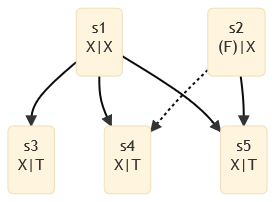
\includegraphics[width=\textwidth,height=5cm,keepaspectratio]{images/reduced_classical.png}
  \caption{Beispielstruktur\label{fig:classset-initial1}}
\end{figure}

 Als Beispiel für den Ablauf kann die folgende Struktur genommen werden:
 \begin{enumerate}
     \item Die Struktur beinhaltet 5 Sätze: $\{s1,...,s5\}$
     \item Aus $s1$ folgen $s3, s4, s5$.
     \item Aus $s2$ folgen $\neg s4, s5$
 \end{enumerate}
 
 Die initialen Überzeugungen ($C_0$) definiere ich wie folgt:
 
 $C_0 = \{s3, s4, s5\}$
 
 Eingängiger ist die Struktur und die initialen Bedingungen auf Abbildung \ref{fig:classset-initial1} dargestellt.\footnote{Die Zeichen unter den Satzbezeichnungen sind wie folgt zu deuten: \textit{Position in der Theorie | Position in den Überzeugungen} Dabei steht X für: \textit{Dieser Satz kommt in der Menge nicht vor}. T für \textit{Dieser Satz ist in der Menge} und F für \textit{Die Negation des Satzes ist in der Menge.} Zusätzliche Klammern (()) können vorkommen um anzuzeigen, dass diese Position notwendig ist, um kohärent zu sein.}
 Unser initialer Epistemischer Zustand $(C_0, T_0)$ ist gegeben durch die leere menge und die oben definierten initialen Überzeugungen. Zur ersten Anpassung der Theorie - Also um $T_1$ zu finden - wird nun die initiale Theorie genommen, und ihr werden einzeln alle Sätze des Themas S hinzugefügt.
 $$
 T_0: \{\} \longrightarrow T_0^*: \{\{s1\},...,\{s5\}, \{\neg s1\}, ..., \{\neg s5\}\}
 $$
 Beim \hyperref[1.1]{zweiten Schritt} kommt keine Menge hinzu, denn in der leeren Menge gibt es keine Sätze, die negiert werden könnten. Auch beim \hyperref[2]{dritten Schritt} kommen keine neuen Sätze hinzu, denn man kann keine Sätze aus der leeren Menge entfernen. Auch im \hyperref[konsistenzfilter]{vierten Schritt} können keine Mengen entfernt werden, denn eine Menge mit einem Element kann nie inkonsistent sein. Die erste Anpassung der Theorie überprüft also einfach alle einzelnen Sätze $\{s1,...,s7, \neg s1, ..., \neg s7\}$. Derjenige, welche den höchsten Wert von $Z$ erreicht, wird zum einzigen Prinzip. Dies ist $s1$, dessen Inhalt $\{s1,s3,s4,s5,\neg s2\}$ ist. Sie erhält die meisten Punkte im Desiderat Kohärenz, denn Sie enthält alle Überzeugungen im Inhalt und keine der Überzeugungen ist inkonsistent mit der Theorie. Einzige Abzüge in der Kohärenz erhält $\{s1\}$ weil sie viele Sätze impliziert, die gar nicht Teil der Überzeugungen sind: $\{s1, \neg s2\}$ sind im Inhalt, aber nicht in den Überzeugungen. Trotzdem erreicht $\{s1\}$ einen höheren Wert bei $Z$ und wird damit zu $T_1$.
 
 Die Überzeugungen müssen als Nächstes angepasst werden. Dazu überprüfen wir die Menge von Mengen, welche $C_0$ und einen weiteren Satz enthalten.
 
 \begin{equation} \notag
 \begin{split}
 C_0^*: \{\{s3, s4, s5, \textcolor{red}{s1}\}, \{s3, s4, s5, \textcolor{red}{s2}\}, \\
 \{s3, s4, s5, \textcolor{red}{\neg s1}\}, \{s3, s4, s5, \textcolor{red}{\neg s2}\}\}
 \end{split}
 \end{equation}
 
 Im Schritt \ref{c1.1} werden dann alle Mengen erstellt, die entstehen, wenn man einzelne Sätze in $C_0$ negiert.
 
 \begin{equation} \notag
 \begin{split}
 C_0^{**}: C_0^* \cup \{\{\textcolor{red}{\neg s3}, s4, s5\}, \{s3, \textcolor{red}{\neg s4}, s5\}, \{s3, s4, \textcolor{red}{\neg s5}\}\}
 \end{split}
 \end{equation}
 
 Ausserdem überprüfen wir entsprechend Schritt \ref{c2} die Mengen, welche entstehen, wenn man einen einzelnen Satz aus $C_0$ entfernt.
 
$$
    C_0^{***}:= C_0^{**} \cup \{ \{s4,s5\}, \{s3,s5\}, \{s3,s4\} \}
$$
 
 Von all den Überzeugungsmengen in $C_0^{***}$ haben folgende 3 Mengen den gleichen Wert der Achievement-Funktion: $\{s3,s4,s5,s1\}$, $\{s3,s4,s5,\neg s2\}$. Ob man also $s1$ zu den weiteren Überzeugungen dazunimmt oder $\neg s2$ hinzunimmt, spielt für die nächste Generation keine Rolle. In allen beiden Optionen wird nämlich das Desideratum der Kohärenz etwas besser erfüllt und das Desideratum des Respekts etwas weniger gut, denn wir haben einen Satz in der Überzeugungsmenge, der nicht zur ursprünglichen Überzeugungsmenge gehört. 
Eine der beiden Möglichkeiten wird nun zufällig ausgewählt. Wir legen uns für das Beispiel fest: $C_1 = \{s3, s4, s5, \neg s2\}$
 
 Bei der zweiten Anpassung der Theorie müssen nun folgende Theoriekandidaten geprüft werden:
\begin{align}
    T_1^{*}:= &\{\{s1, s3\}, \{s1, s4\}, \{s1, s5\},\stkout{\{s1, s2\}}, \{s1, \neg s2\}, \stkout{\{s1, \neg s3\}, \{s1, \neg s4\}, \{s1, \neg s5\}}\}\\
    T_1^{**}:= T_1^{*} \cup &\{\{\neg s1\}\}\\
    T_1^{***}:= T_1^{**} \cup &\{\{\}\}
\end{align}
Die durchgestrichenen Kandidaten werden in Schritt \ref{konsistenzfilter} entfernt, weil sie inkonsistent mit $\{s1\}$ sind.
 Das Resultat ist, dass keine der überprüften Theorien besser ist als $T_1$. Somit wird $T_1$ auch zu $T_2$ übernommen.
 
 Es folgt eine weitere Anpassung der Überzeugungen. Wir erinnern uns, dass wir im letzten Anpassungsschritt die Wahl zwischen der Hinzufügung von $s1$ zu $C_0$ hatten oder der Hinzufügung von $\neg s2$. Wir hatten und zufällig für die zweite Option entschieden. Da sich die Theorie im letzten Anpassungsschritt nicht verändert hat, liegt auf der Hand, dass das Hinzufügen von $s1$ zu $C_1$ die beste Alternative sein muss. Ich überspringe an dieser Stelle also das aufzeichenn und vergleichen von $C_1^{***}$ und füge $s1$ zu $C_1$ hinzu. Somit sieht $C_2$ nun wie folgt aus: $C_2 = \{s3, s4, s5, \neg s2, s1\}$
 
 Weil $T_2$ mit $T_1$ identisch ist, müssen im nächsten Theorieanpassungsschritt um $T_3$ zu finden auch dieselben Theoriekandidaten überprüft werden. Da die Hinzufügung von $s1$ zu den Überzeugungen optimal für $T_2$ war, kann es keine Theorie geben, die besser passt. Denn wäre das der Fall, so müssten wir in einem der vorherigen Theorieanpassungsschritte eine suboptimale Theorie ausgewählt haben. Das führt mich zur Annahme, dass bei einer dialektischen Struktur mit einder Prämisse, keine weiteren Theorieanpassungsschritte unternommen werden müssen, wenn in einem Schritt keine bessere Theorie gefunden wurde. Dafür benötigt es natürlich einen Beweis oder wenigstens weitere experimentelle Hinweise, deshalb lasse ich dies als Vermutung hier stehen. Für das Beispiel lässt sich aber feststellen, dass es keine bessere Theorie als $\{s1\}$ gibt. $T_3$ ist daher $\{s1\}$.
 
 Es folgt eine letzte Überprüfung der Überzeugungen. Folgende Mengen werden überprüft:
 \begin{align}
    C_2^{*}:= &\{\}\\
    C_2^{**}:= C_2^{*} \cup &\{\{\neg s3, s4, s5, \neg s2, s1\}, \{s3, \neg s4, s5, \neg s2, s1\}, \{s3, s4, \neg s5, \neg s2, s1\},\\ \notag
    &\{s3, s4, s5, s2, s1\}, \{s3, s4, s5, \neg s2, \neg s1\}\}\\
    C_2^{***}:= C_2^{**} \cup &\{\{s3, s4, s5, \neg s2\}, \{s3, s4, s5, s1\}, \{s3, s4, \neg s2, s1\}, \{s3, s5, \neg s2, s1\},\\ \notag
    &\{s4, s5, \neg s2, s1\}\}
 \end{align}
 
 Dabei fällt auf, dass mit $C_2^{*}$ keine neuen Kandidaten gefunden werden können. Denn jeder Satz in S kommt schon (evtl. negiert) in $C_2$ vor. Dafür werden in den folgenden Schritten jeweils $\lvert S \rvert = 5$ Mengen gefunden, welche überprüft werden müssen.
 Nach dem beschriebenen Rezept wird diese wieder durchgeführt, mit dem Ergebnis, dass es keine Verbesserung gibt und $C_3$ mit $C_2$ gleichgesetzt wird. Weil bei der letzten Theorieanpassung schon keine bessere Theorie gefunden wurde, ist damit die Stoppbedingung erfüllt und der Prozess endet in einem Reflective Equilibrium.
 
 Während des Prozesses mussten in den drei Theorieanpassungsschritten 22 Theoriekandidaten (30 Kandidaten - 8 inkonsistente Mengen) überprüft werden.  Im Vergleich zum traditionellen Ansatz, bei dem in jedem Schritt $3^5$ Mengen (abzüglich der inkonsistenten Theoriekandidaten) überprüft und verglichen werden müssen. In der Anpassung der Überzeugungen im Beispiel müssen bei allen drei Anpassungen insgesamt 30 Überzeugungen überprüft werden. Beim traditionellen Ansatz müssen bei jedem Schritt wieder $3^5$ Überzeugungen überprüft werden. Wichtig für die Frage, ob der traditionelle Ansatz wirklich weniger effizient ist, ist neben der Anzahl zu überprüfenden Mengen pro Schritt auch die Anzahl der Schritte. Diese wäre für unser Beispiel für das traditionelle Modell bei beiden Anpassungen 3 Schritte, für den neuen Ansatz sind es auch je 3 Schritte. Die Anzahl Schritte ist also tatsächlich gleich hoch, aber die Anzahl von hinzugefügten Mengen pro Schritt ist $48.6$ mal tiefer im piecemeal Ansatz. Wenn sich bei weiteren Kompositionen ähnliche Werte ergeben, ist die neue Methode der traditionellen vorzuziehen. Ausserdem gilt es zu überprüfen, ob die Methode globale Optima erreicht. Ausserdem gibt es für piecemeal einige weitere Einschränkungen und Schwierigkeiten, auf die ich noch zu sprechen komme.
 % Run the numbers again...

\section{Ensemblestudie} \label{Ensemblestudie}

Um zu untersuchen, wie sich der Piecemeal-Ansatz gegenüber dem Standard-Ansatz verhält, habe ich ein umfangreiches Datenset generiert und dieses analysiert. Ich werde in diesem Abschnitt kurz darauf eingehen, wie das Datenset aufgebaut ist und dann erklären, was ich untersucht habe und was die Erkenntnisse sind. Generiert wurden die Daten alle mittels einer Python-Bibliothek, wie von den Mitgliedern des Forschungsprojekts \textit{How Far Does Reflective Equilibrium Take Us?} erarbeitet wurde.

\paragraph{Die Bewertungskriterien} Wie gut sind die Fixpunkte? 

\paragraph{Aufbau} Ich habe 2400 RE-Prozesse generiert. Davon sind die Hälfte Prozesse nach dem neuen Piecemeal-Ansatz und die andere Hälfte nach dem Standard-Ansatz. Angefangen bei einer Menge von fünf Sätzen im Satzpool wurden jeweils 50 zufällige Argumentstrukturen generiert und mit 2 zufällig generierten Mengen von initialen Überzeugungen kombiniert. Der Prozess wird wiederholt und diesmal werden auch Argumente mit bis zu zwei Prämissen erlaubt. Dies wurde für Poolgrössen von 5 bis 10 wiederholt, was 1200 initiale Strukturen ergibt. Alle wurden mit dem Standard-Prozess und mit dem Piecemeal-Vorschlag untersucht, was dann 2400 RE-Prozesse ergibt.

\paragraph{Anzahl der initialen Überzeugungen} Es fällt auf, dass drei Viertel der Prozesse, welche dieselben initialen Strukturen haben, unterschiedliche Fixpunkte erreichen. Wenn man davon ausgeht, dass der Standard-Ansatz eigentlich immer ein globales Optimum erreicht, würde das bedeuten, dass der Piecemeal-Ansatz in diesen Fällen bei einem Fixpunkt stehen bleibt, der einen schlechteren Wert bei der Funktion Z erreicht. Dass dies nicht unbedingt so ist, lässt sich in Grafik \ref{fig:höheres Achievement aufgeteilt nach initialen Commitments} zeigen: Je nachdem, wie viele initiale Überzeugungen in der initialen Struktur waren, kann der Piecemeal-Ansatz durchaus bessere Ergebnisse erreichen. Bei nur einem oder zwei initialen Überzeugungen funktioniert der Standard-Ansatz immer besser. Je höher die Zahl der Überzeugungen am Anfang des Prozesses aber wird, umso besser funktioniert auch der Piecemeal-Ansatz.

\begin{figure}[ht]
  \centering
  \includegraphics[width=\textwidth]{höheres Achievement aufgeteilt nach initialen Commitments}
  \caption{höheres Achievement aufgeteilt nach initialen Überzeugungen A\label{fig:höheres Achievement aufgeteilt nach initialen Commitments}}
\end{figure}

\begin{figure}[ht]
  \centering
  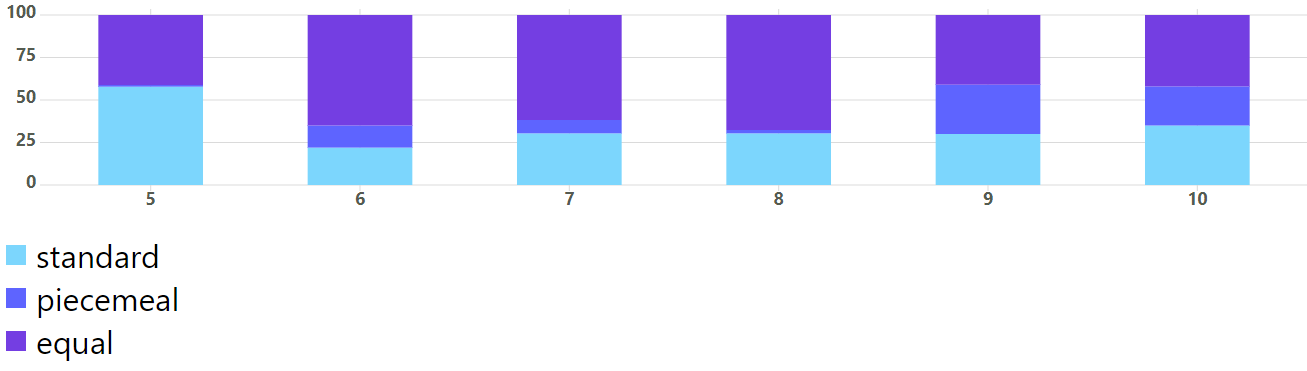
\includegraphics[width=\textwidth]{höheres Achievement aufgeteilt nach Poolsize begrenzt auf eine Prämisse}
  \caption{höheres Achievement aufgeteilt nach Poolsize begrenzt auf ein-Prämisse-Strukturen\label{fig:höheres Achievement aufgeteilt nach Poolsize begrenzt auf eine Prämisse}}
\end{figure}

\begin{figure}[ht]
  \centering
  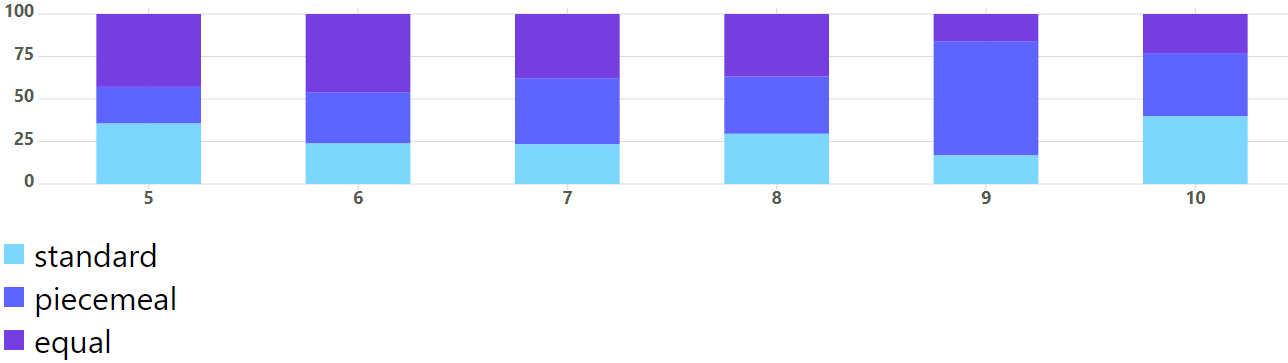
\includegraphics[width=\textwidth]{höheres Achievement aufgeteilt nach Poolsize begrenzt auf max 2 Prämissen}
  \caption{höheres Achievement aufgeteilt nach Poolsize begrenzt auf 2 Prämissen-Strukturen\label{fig:höheres Achievement aufgeteilt nach Poolsize begrenzt auf max 2 Prämissen}}
\end{figure}


In den Grafiken \ref{fig:höheres Achievement aufgeteilt nach Poolsize begrenzt auf eine Prämisse} und \ref{fig:höheres Achievement aufgeteilt nach Poolsize begrenzt auf max 2 Prämissen} ist erkennbar, dass der Piecemeal-Ansatz deutlich besser funktioniert, wenn die Argumente 2 Prämissen haben können und die grösse des Satzpools etwas grösser ist als nur 5. Wie dies sein kann, möchte ich anhand eines Schritt-für-Schritt-Beispiels einer initialen Struktur zeigen. Welche zufällig generiert wurde:

\textit{\textcolor{red}{Hier fehlt das Schritt-für-Schritt-Beispiel}}

\begin{figure}[ht]
  \centering
  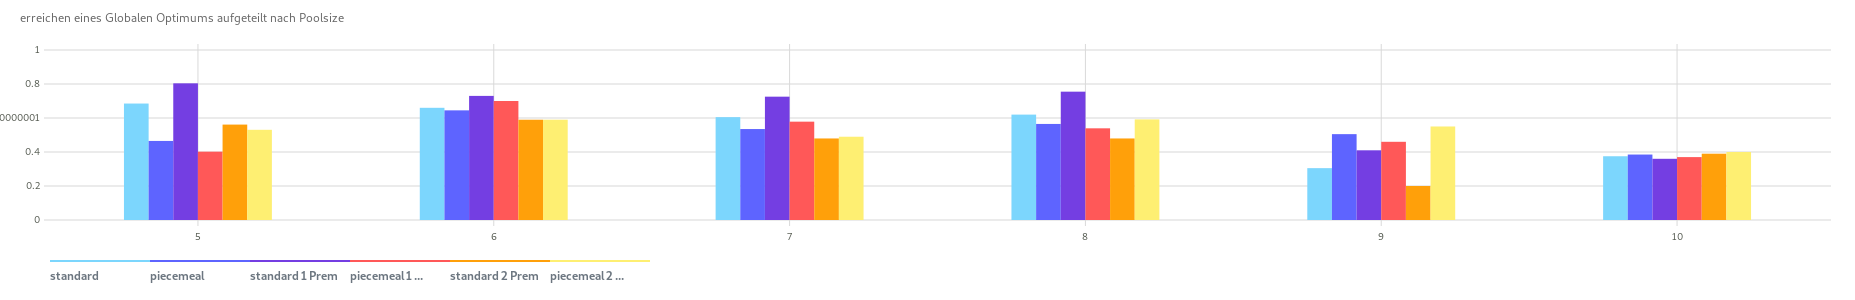
\includegraphics[width=\textwidth]{erreichen eines Globalen Optimums aufgeteilt nach Poolsize}
  \caption{erreichen eines Globalen Optimums aufgeteilt nach Poolsize\label{fig:GlobOptPoolsize}}
\end{figure}


Wenn man Grafik \ref{fig:GlobOptPoolsize} analysiert, so erkennt man, dass die Standard-Variante zwar meistens die Nase vorn hat, dies jedoch nur, weil er bei Argumenten mit nur einer Prämisse wesentlich besser funktioniert. So erreicht er denn bei Argumenten mit einer Prämisse und einer Poolgrösse von 5 zu 80\% das globale Optimum im Vergleich zu Argumenten mit einer Prämisse, wo es nur 56\% sind. Schaut man sich die zweiprämissigen Argumente an, so erreicht Piecemeal schon ab einer Poolgrösse von 6 öfter ein globales Optimum.

Warum die Anzahl an Argumenten Einfluss auf die Leistungsfähigkeit des Ansatzes hat, kann ich nicht mit Sicherheit sagen. Was die Analyse allerdings zeigt, sofern meine Daten richtig sind, dass der Standard-Ansatz nicht so robust ist, wie \autocite[S.~17-18]{beisbart_making_2015} behaupten. In ihren untersuchungen verändern \citeauthor{beisbart_making_2015} die Gewichtungen der Achievmentfunktion und die Überzeugungen, nicht aber die Argumentstruktur und die Menge der Sätze. Die erreichten 95\% von Prozessen, die ein globales Optimum erreichen, kann ich mit den von mir erstellten Daten nicht annähernd nachweisen.

\textit{\textcolor{red}{Ich werde noch mehr dazu erzählen wie die Grafiken entstanden sind. Dabei werde ich nicht auf Programmcode zurückgreifen, sondern einfach erklären, welche Werte ich wann wie gefiltert habe, damit der Leser verstehen kann, was die Diagramme darstellen.}}

Alle Grafiken können als interaktive SVGs auf dieser Website abgerufen werden: \href{https://piecemeal.flicks.jetzt/}{piecemeal.flicks.jetzt}

\subsection{Entdeckte Probleme}
\paragraph{Falsche Reihenfolge der Anpassungen} Der Programmierte Ansatz funktioniert nicht genau wie der Prozess, den ich in Absatz \ref{piecemealansatz} definiert habe. Der wichtigste unterschied ist folgender: Die Reihenfolge in der die Schritte unternommen werden, ist vertauscht. Sie sieht wie folgt aus:
\begin{enumerate}
    \item $C_0$ wird definiert aus den eingegebenen Überzeugungen.
    \item $T_0$ wird als leere Menge definiert.
    \item Die Überzeugungen passen sich an die aktuelle Theorie an.
    \item Die Theorie passt sich an die aktuellen Überzeugungen an.
    \item Die beiden vorherigen Schritte werden wiederholt, bis die Stoppbedingung eintrifft.
\end{enumerate}

Diese Reihenfolge führt dazu, dass immer die Menge der Überzeugungen an die leere Menge angepasst wird. Was in jedem Fall dazu führt, dass ein zufälliger Satz aus der Menge der Überzeugungen gestrichen wird. Dies kann natürlich nur hinderlich sein. Im besten Fall führt es zu einigen zusätzlichen Anpassungsschritten, im schlechtesten Fall zu einem intuitiv nicht nachvollziehbaren Ergebnis.

\begin{figure}[ht]
  \centering
  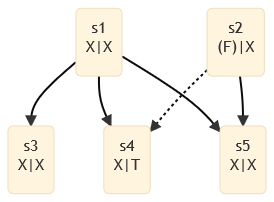
\includegraphics[width=\textwidth,height=5cm,keepaspectratio]{images/wierd.png}
  \caption{Struktur, die zu einem nicht nachvollziehbaren Ergebnis führt.\label{fig:wierd}}
\end{figure}

Betrachten wir die Struktur, die in Abbildung \ref{wierd} abgebildet ist. Wenn die Menge der Überzeugungen nur ein Element enthält - wie in unserem Fall $s4$, bedeutet das, dass sich nach dem ersten Anpassungsschritt an die initiale Theorie - welche die leere Menge ist - die leere Menge auch als Überzeugungsmenge ergibt. An die leere Menge passt sich dann die leere Menge der Theorie an und wählt einen zufälligen Satz, aus dem keine anderen Sätze folgen, aus. Warum wird nicht die leere Menge beibehalten? Sie erreicht ja volle Kohärenz, denn der Inhalt enthält alle und nur die Sätze in der Überzeugungsmenge - keine. Weil die Systematizität der leeren Menge immer 0 ist und somit irgendein Satz besser ist als die leere Menge. Warum sollen aus dem Satz keine anderen Sätze folgen? Weil, wie im Absatz \ref{achievement-funktion} erklärt, es in der Kohärenz Abzüge gibt, für jeden Satz im Inhalt der Theorie, welcher nicht auch in den Überzeugungen enthalten ist. Sätze, aus denen keine anderen Sätze folgen,  enthalten im Inhalt lediglich sich selbst.
Die Überzeugungen passen sich danach wieder an den zufällig gewählten Satz an und übernehmen diesen. Das heisst, dass am Ende des Prozesses entweder $s3$, $s4$ oder $s5$ als alleiniger Satz in der Theorie und Überzeugung dastehen. Dies ist enorm kontraintuitiv.

Wie kann das Problem gelöst werden? Die eine offensichtliche Antwort lautet, dass das Programm die Reihenfolge einhalten kann, welche ich in meinem Ansatz definiert habe. Noch viel wichtiger scheint mir aber, eine bessere erste Theorie als die leere Menge zu finden. Ein Ansatz dafür befindet sich im Anhang. Eine andere Möglichkeit wäre es, $T_0 := C_0$ zu setzen.

\paragraph{Globale Optima werden verfehlt} Es ist möglich, sich Strukturen auszudenken, die mit dem piecemeal Ansatz nicht optimal gelöst werden und die der standard Ansatz besser löst. Sehen wir uns folgendes Beispiel an:


\section{Fazit}

Aufwand von Piecemeal viel besser... 


\newpage
\printbibliography

\newpage

\section{Anhang}
\subsection{ Vorschlag für eine erste Theorie: Analyse der Inferenzbeziehungen} \label{better-first-theory}
Im traditionellen Ansatz wird im initialen Zustand die leere Menge als erste Theorie angenommen. Ich möchte einen alternativen Vorschlag vorstellen, wie eine erste Theorie gefunden werden könnte. Er entstand durch die Überlegung, wie Personen den Prozess wohl intuitiv durchführen würden. Die Idee ist, dass man sich die Inferenzbeziehungen der Argumente anschaut, welche die ersten Überzeugungen beinhalten. Aufgrund der Inferenzbeziehungen zwischen Sätzen, kann klug entschieden werden, welche Sätze sich eher als Theorien lohnen. Es gilt zu beachten, dass bei der Analyse der Inferenzbeziehungen ignoriert wird, dass Sätze auch Prinzip für sich selbst sein können. Dies dürfte aber kein Problem sein bei der Erstellung einer ersten Theorie.

\paragraph{Generierung der Theorie}
Ausgehend von der Menge von Überzeugungen $C_0$ wird eine Theorie $T_0$ wie folgt erzeugt. Wann immer eine Menge mit Subskript angegeben wird, ist damit der Wert in der Menge mit dem Index des Subskripts gemeint.
\begin{enumerate}
    \item Zu Beginn des Prozesses hat der Index $z$ - welchen wir benötigen werden um durch die Mengen in $P$ zu iterieren - den Wert Null. Und die Menge $S$ - welche unsere Theoriekandidaten enthält - entspricht am Anfang der leeren Menge. $S = \{\}$ $z = 0$
    \item Die Menge $P$ wird aus $C_0$ generiert. Sie enthält die alle Permutationen von $C_0$. $P$ ist indexiert.
    $$
        P := \{ M_i : M_i \text{ ist eine Permutation von } P\}
    $$
    \item \label{i1} Die erste Überzeugung aus der Menge in $P_z$ wird ausgewählt: $a = 0$ (Index 0)
    \item \label{i2} Falls die Menge $S_z$ leer ist: Für die aktuell ausgewählte Überzeugung $P_z^a$ werden alle Prinzipien gesucht, aus welchen die ausgewählte Überzeugung folgt. Jedes gefundene Prinzip eröffnet eine neue Menge und diese Mengen werden $S_z$ hinzugefügt. Falls $S_z$ nicht leer ist: Jedes für $P_z^a$ gefundene Prinzip wird zu den Mengen in $S_z$ hinzugefügt, falls die entstehende Menge konsistent ist und das Prinzip nicht schon enthalten ist.
    \item \label{i3} Falls $P_z^a$ noch nicht das letzte Element aus $P_z$ ist, wird die nächste Überzeugung aus $P_z$ ausgewählt (indem a um Eins inkrementiert wird) und zu Schritt \ref{i2} gesprungen.
    $$
        a = a + 1
    $$
    \item \label{i4} Falls $z < \lvert C_i \rvert!$ : $z$ wird um eins inkrementiert: $z = z + 1$ und zu Schritt \ref{i1} gesprungen.
    \item \label{i5} In den Mengen $S$ werden die Mengen, welche die gleichen Elemente enthalten, zu einer reduziert. Alle $S$ Mengen werden mittels Achievement-Funktion $Z$ überprüft.
    \item \label{i6} Die Theorie, welche den höchsten Wert bei $Z$ erreicht, wird zur Theorie $T_0$. Falls mehrere Theorien den höchsten Wert erreichen, wird eine Theorie zufällig ausgewählt.
\end{enumerate}

\paragraph{Beispiel}
Beispielhaft kann auch hier wieder die Struktur, welche auf Abbildung \ref{fig:classset-initial1} illustriert ist, dienen. Im ersten Schritt wählen wir $s3$ und finden $s1$ als mögliches Prinzip für $s3$ im zweiten Schritt. Da $S_0$ noch leer ist, fügen wir $s1$ hinzu. Dann suchen wir ein Prinzip für $s4$, wobei wir wieder auf $s1$ stossen und dieses nicht ein zweites Mal zu $S_0$ hinzufügen. Danach folgt unsere nächste und letzte Überzeugung $s5$. Für $s5$ finden wir nun zwei mögliche Prinzipien: $s1$ und $s2$. Nun ergäben sich zwei Mengen in $S_0$: $\{s1\}$ und $\{s1, s2\}$. Da $\{s1, s2\}$ aber inkonsistent ist, wird sie weggelassen. Als Nächstes starten wir den Prozess erneut, diesmal fangen wir aber mit $s4$ als erster Überzeugung an, für die wir Prinzipien suchen. Der Prozess verläuft analog zum ersten Durchgang, und am Ende haben wir eine Menge $S_1 = \{s1\}$. Für den dritten und letzten Durchgang mit $s5$ als Startüberzeugung ergibt sich aber ein anderes Bild: Zu $S_2$ werden die beiden Prinzipien $s1$ und $s2$ als einzelne Elemente hinzugefügt. Bei der Suche nach einem Prinzip für $s4$ und analog für $s3$ wird jeweils $s1$ gefunden. Zur ersten Menge in $S_2$ wird $s1$ nicht hinzugefügt, weil es schon darin ist, zur zweiten Menge nicht, weil die resultierende Menge $\{s1,s2\}$ inkonsistent wäre. Somit ist $S_1 = \{{s1}, {s2}\}$. Die Mengen in $S_0$, $S_1$ und $S_3$ werden nun zusammengeführt, wobei die Doppelungen wieder gestrichen werden können. Somit ergeben sich folgende Kandidaten, für die ihr $Z$-Wert verglichen werden muss: $\{\{s1\}, \{s2\}\}$.

\paragraph{Aufwand}
Da alle Permutationen von $C_0$ durchlaufen werden müssen, umfasst die Methode relativ viele Schritte. Allerdings gäbe es vielleicht eine Möglichkeit, nicht über alle Permutationen iterieren zu müssen und beispielsweise nur mit jedem Element aus $C_0$ einmal anzufangen. Dies bedarf aber weiterer Forschung und ist nicht Gegenstand dieser Arbeit.

\end{document}


%%%%%%%%%%%%%%%%%%%%%%%%
\subsubsection{piecemeal Inferenzanalyse}

Eine interessante Alternative zur Inferenzanalyse ist die Idee, die Anpassung der Theorie auch schrittweise zu machen. Dies würde einerseits einen weiteren piecemeal-Aspekt umsetzen und andererseits das Problem der Notwendigkeit der Permutation der Überzeugungen lösen. Die Theorieanpassung würde wie folgt aussehen:

\begin{enumerate}
    \item Die erste Überzeugung aus $C_i$ wird ausgewählt: $c_a = c_0$ (Index 0)
    \item Für die ausgewählte Überzeugung $c_a$ werden alle Prinzipien gesucht, welche die ausgewählte Überzeugung zum Inhalt haben. Jedes gefundene Prinzip wird $S$ hinzugefügt, wenn es nicht schon in der Menge enthalten ist.
    \item Falls $c_x$ noch nicht das letzte Element aus $C_i$ ist, wird die nächste Überzeugung aus $C_i$ ausgewählt und zu Schritt \ref{i2} gesprungen.
    \item Aus den Elementen in $S$ werden alle konsistenten Mengen gebildet.
    \item Diese Mengen werden mittels Achievement-Funktion $Z$ überprüft.
    \item Die Theorie, welche den höchsten Wert bei $Z$ erreicht, wird zu $T_{i+1}$ erklärt, falls ihr $Z$-Wert auch grösser ist als jener von $T_i$ - Ansonsten wird $T_i$ zu $T_{i+1}$.
\end{enumerate}


\begin{enumerate}
    \item How can logic be defined in a general way, so that different rival theories can be understood as \textit{logical} theories?
\end{enumerate}

\begin{quote}
    An argument is logically valid just when conditional [sic.], with the conjunction of the premises as antecendent and the conclusion as consequent, is logically true. We can readily slip from one notion to the other[...] \cite[p.~13]{beallrestall}
\end{quote}

\subsection{Debating on logic}\label{sec:debating}
\footnote{An extensive discussion of trivialism and why it is an irrational view can be found in chapter 3 of \citeA{priest2}.}

 \fullciteauthor{beallrestall}

(see section \ref{principle:GGTP}, page \pageref{principle:GGTP})

\begin{center}
\begin{tabular}{c p{9cm}}
P1 & If I am king of France, I'm not king of France.\\\hline
C & If I am king of France, God exists. 
\end{tabular}
\end{center}

\paragraph{Systematicity} To define the consequence relation by specifying it for each argument separately would be a very unsystematic procedure. \textbf{Systematicity}, like the one brought forward by \citeauthor{resnik0} or \citeauthor{peregrinsvoboda}. They have, as I will argue, a problematic understanding of the purpose of an RE-process.